\section{Contexto}
\label{sec:Prop_Contexto}

En este capítulo se presentan los \textbf{aportes} (son aportes? algunas cosas solo las vamos a usar no mejorar) en los diferentes aspectos del ciclo de vida del contexto presentado por Perera et al. \cite{Perera2014}. En la sección \ref{subsec:Prop_Modelado} se definen los componentes ontológicos con los que se representará el contexto mientras que en las secciones \ref{subsec:Prop_Adquisicion}, \ref{subsec:Prop_TransDatos} \ref{subsec:Prop_Razonamiento} y \ref{subsec:Prop_Servicio} se presentan a detalle los componentes del modelo de la figura \ref{fig:Diagrama_Contexto}, este modelo tiene en cuenta trabajos del estado del arte en razonamiento y modelado del contexto (CITAS) y está compuesta por las siguientes capas: (CÓMO PONERLE QUE EL MODELO ES DEL PROCESO DE CONTEXTO SIN REPETIR TANTO?)

\begin{itemize}
    \item Captura de datos: Capa dedicada a la adquisición de los datos relevantes para el sistema de contexto, tiene en cuenta las entidades que intervienen en la interacción, los contenidos multimedia y los datos obtenidos de fuentes externas. Adicionalmente se encarga de limpiar y organizar la información para su posterior transformación.
    \item Transformación de datos: Transforma la información al formato RDF permitiendo la interoperabilidad con otros sistemas y facilitando el uso de redes semánticas para la descripción del contexto del usuario.
    \item Razonamiento: Analiza los datos capturados para encontrar el contexto que describe las situaciones de un usuario, cuenta con un conjunto de reglas relevantes según cada uno de los usuarios, asegurando la personalización en los servicios a proveer.
    \item Servicio: Presenta al usuario los servicios identificados en la etapa de razonamiento, tiene en cuenta los dispositivos de interacción y los gustos y necesidades del usuario. Este componente se verá afectado por las actividades que el usuario requiere haga el sistema.
\end{itemize}

% \begin{figure}[ht]
% \centering%
% \includegraphics[width=\textwidth]{Cap3/Diagrama_Contexto}%
% \caption{Arquitectura de contexto MCARS.} \label{fig:Diagrama_Contexto}
% \end{figure}

\begin{figure}[ht]
\centering%
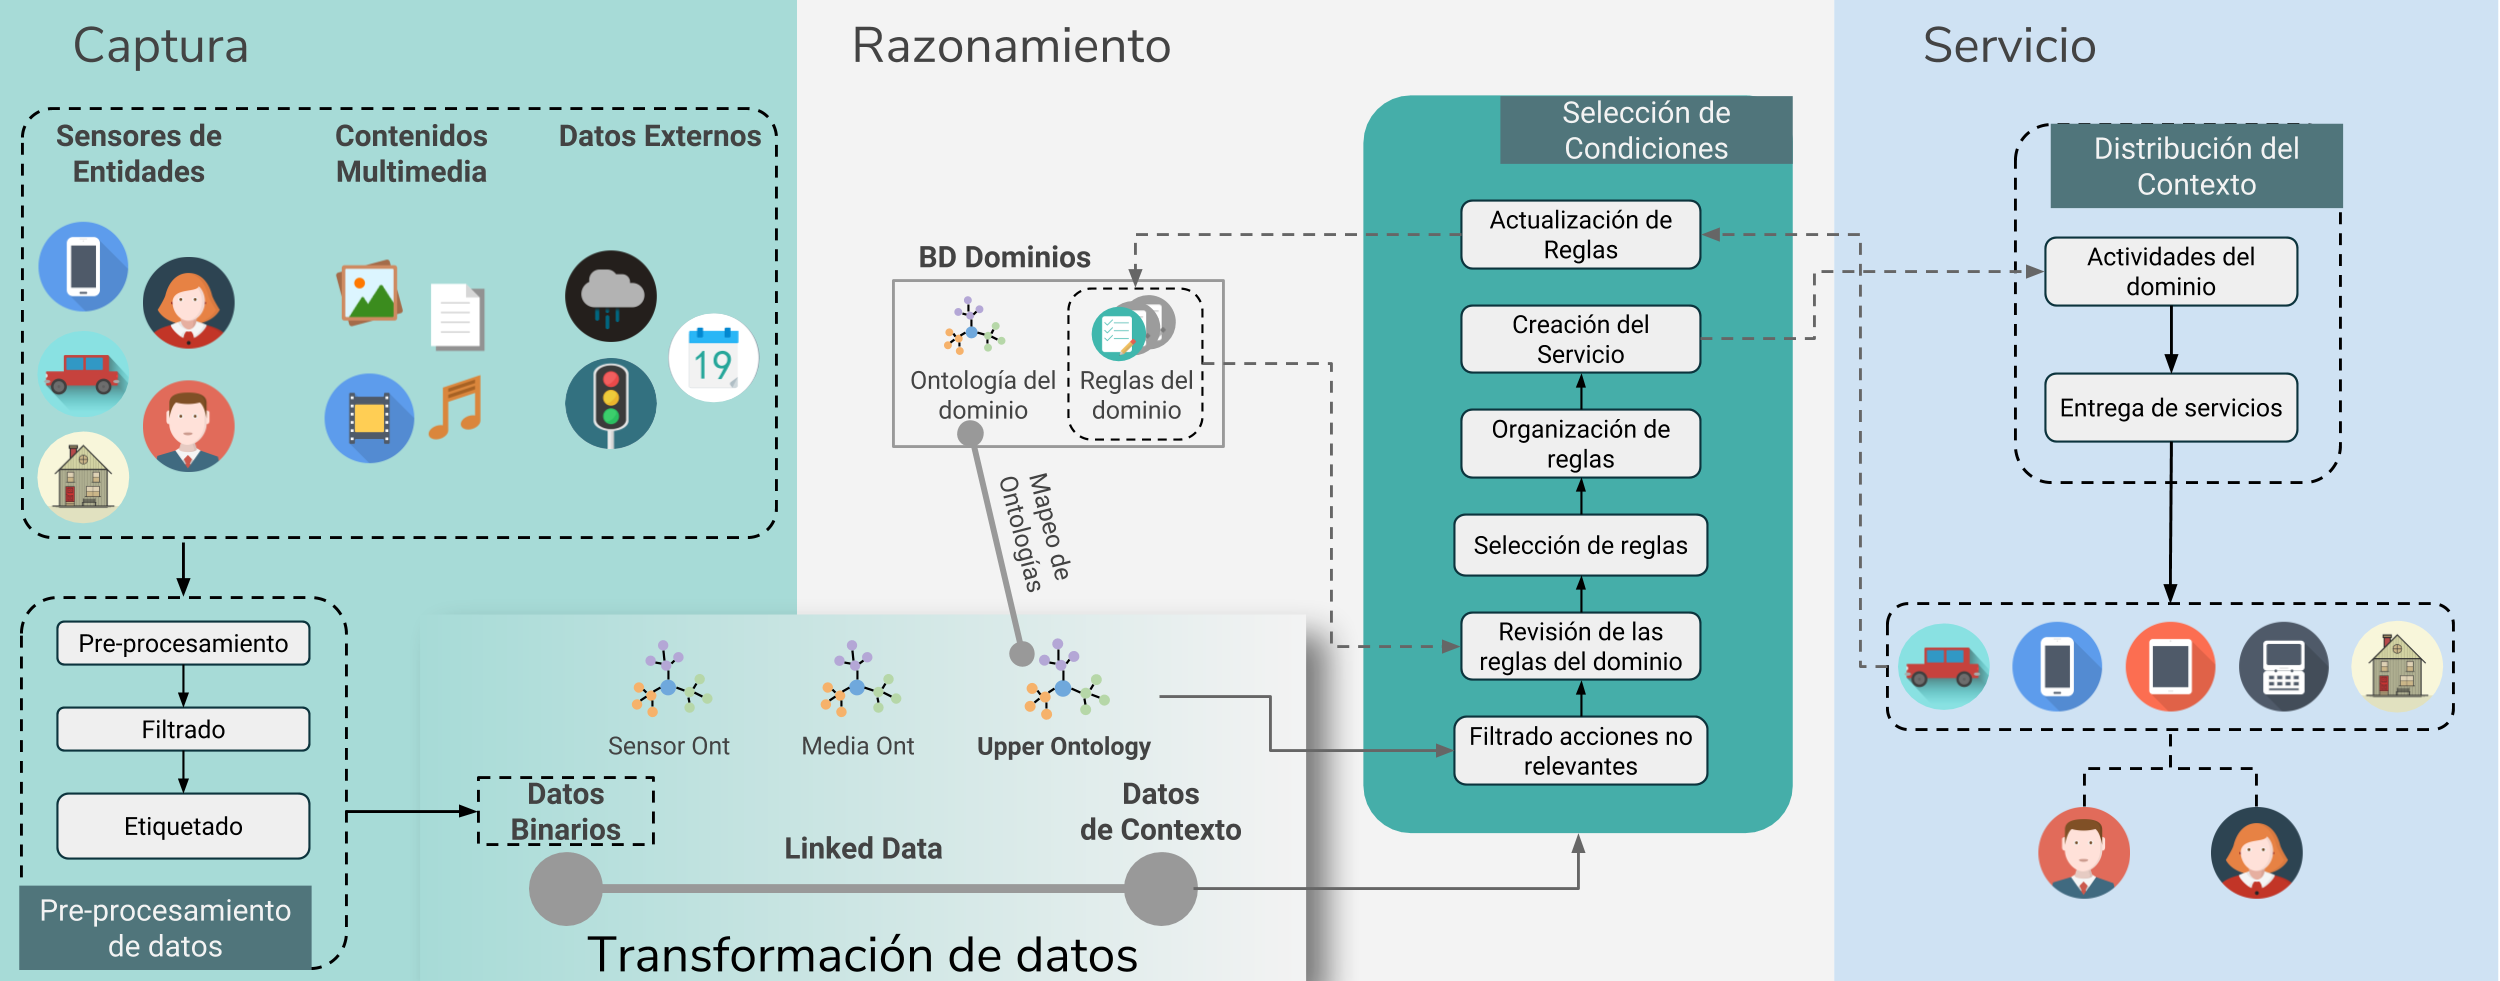
\includegraphics[width=\textwidth]{Cap3/Images/Diagrama_Contexto_v2}%
\caption{Arquitectura de contexto MCARS.} \label{fig:Diagrama_Contexto}
\end{figure}


\cite{Avenoglu2017} dice que separar la administración del contexto y las operaciones de adaptación al contexto permite especializar el sistema.